The previous two chapters described the background for RL and DL. In this chapter, we will see 
how these two fields are combined in powerful state-of-the-art algorithms for solving complex reinforcement learning problems.
In this work, we use all the algorithms presented in this chapter.

\section{Deep Deterministic Policy Gradients (DDPG)}

DDPG \cite{DDPG} is an off-policy actor-critic algorithm that simultaneously estimates the policy and the action-value function.
It has two major components (denoted by the actor and the critic):

\begin{itemize}
    \item Actor function $\mu(s \vert \theta^\mu) $ that represents the current policy, mapping states to specific actions.
     It is a policy function approximator using deep neural networks.
    \item Critic function $ Q(s, a \vert \theta^Q)$ that approximates the Q function. 
    It is value function approximator using deep neural networks.
\end{itemize}

DDPG is an extension of the Deterministic Policy Gradient Algorithm (DPG) \cite{DPG}. 
DPG introduces a very important theorem for policy gradient methods that extends the standard policy gradient
theorem for stochastic policies to deterministic policies.

The theorem states: 

% Explain the theorem better

\begin{equation}
\begin{split}
    \nabla_{\theta^\mu} \mu
        & \approx \mathbb{E}_{s_t \sim \mu'}
                [\nabla_{\theta^\mu} Q(s, a \vert \theta^Q)\vert_{s=S_t,a=\mu(S_t \vert \theta^\mu)}]  \\
        & = \mathbb{E}_{s_t \sim \mu'}
                [\nabla_a Q(s, a \vert \theta^Q)\vert_{s=S_t,a=\mu(S_t)}
                \nabla_{\theta_\mu}\mu(s\vert\theta^\mu)\vert_{s=S_t}]
\end{split}
\label{eq:dpg}
\end{equation}

Equation (\ref{eq:dpg}) proves that a deterministic policy gradient can be estimated by the estimated
action-value function's gradient.
DDPG's policy update is based on Equation (\ref{eq:dpg}) and adapts some key ideas from Deep Q-Networks (DQN) \cite{RLNature2015}:
DQN introduces 2 modifications to standard Q-learning algorithm to make it suitable for training
large neural networks without diverging.

\begin{itemize}
    \item Use of a technique known as experience replay. It consists of storing the agent's experiences at each timestep in a 
    dataset so that during the Q-learning updates (inner loop of Algorithm \ref{algo:ddpg}) we use samples of experiences.
    This approach allows for greater data efficiency and the randomization breaks the correlations between temporal data.
    \item Use a copy of the actor and critic as target networks. The target network is updated at a lower frequency
    using the weights of the network $Q$. This improves stability compared to standard Q-learning.
\end{itemize}

DDPG is based on Equation (\ref{eq:dpg}) and uses these ideas from \cite{RLNature2015} applied to the continuous domain.
A major challenge, however, of learning in continuous action spaces is exploration. DDPG and other off-policy algorithms
can explore independently from learning. DDPG employs an exploration policy $\mu'$ by adding noise sampled from a noise process
$\mathcal{N}$ to the actor policy according to:

\begin{equation}
    \mu'(S_t) = \mu(S_t \vert \theta^\mu) + \mathcal{N}
\end{equation}

A novel approach that tackles the problem of action exploration is adding noise to the parameter space,
instead of on the action space \cite{OpenAIParameterNoise}. This is done by adding adaptive noise to
the parameters of the neural network policy and this helps algorithms better explore their environments.
We use this type of exploration in this work.
Figure \ref{fig:parameter_noise} illustrates the differences between action space and parameter space noise.

\begin{figure}[thb]
    \centering
    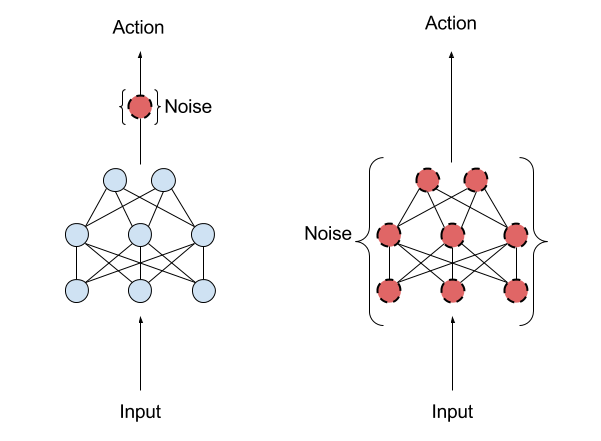
\includegraphics[width=0.6\textwidth]{Chapter4/parameter_noise.png}
    \caption{Comparison between action space noise (left) and parameter space noise (right).
    Extracted from \cite{OpenAIParameterNoise}.}
    \label{fig:parameter_noise}
\end{figure}

Algorithm \ref{algo:ddpg} describes DDPG.

\begin{algorithm}[H]
    \DontPrintSemicolon
    \SetAlgoLined
    % \KwResult{Trained policy \theta^{\mu}}
    Randomly initialize critic network $Q(s, a \vert \theta^Q)$ and actor $\mu(s \vert \theta^\mu)$ 
    with weights $\theta^Q$ and $\theta^\mu$. \;
    Initialize target network $Q'$ and $\mu'$ with weights $\theta^{Q'} \leftarrow \theta^Q$, $\theta^{\mu'} \leftarrow \theta^\mu$.\;
    Initialize replay buffer $R$. \;
    \For{episode = $1$, $M$}{
        Initiliaze a random process $\mathcal{N}$ for action exploration. \;
        Receive initial observation state $S_t$. \;
        \For{t = $1$, $T$}{
            Select action $A_t = \mu(S_t \vert \theta^\mu) + \mathcal{N}_t$ according to the current policy and exploration noise.\;
            Execute action $A_t$ and observe reward $R_t$ and observe new state $S_{t+1}$.\;
            Store transition $(S_t, A_t, R_t, S_{t+1})$ in $R$. \;
            Sample a random minibatch of $N$ transitions $(S_i, A_i, R_i, S_{i+1})$. \;
            Set $y_i = r_i + \gamma Q'(S_{i + 1} , \mu'(S_{i + 1} \vert \theta^{\mu'}) \vert \theta^{Q'})$. \;
            Update critic by minimizing the loss: $L = \dfrac{1}{N} \Sigma_i(y_i - Q(S_i, A_i \vert \theta^Q))^2$. \;
            Update the actor policy using the sample policy gradient: \;
            \Indp\Indp
                $ \nabla_{\theta^\mu}J \approx  \dfrac{1}{N} \nabla_a Q(s, a \vert \theta^Q)\vert_{s=S_t,a=\mu(S_t)}
                \nabla_{\theta_\mu}\mu(s\vert\theta^\mu)\vert_{s=S^t}]$ \;
            \Indm\Indm
            Update the target networks: \;
            
            \Indp\Indp
                $\theta^{Q'} \leftarrow \tau \theta^Q + (1 - \tau)\theta^{Q'}$ \;
                $\theta^{\mu'} \leftarrow \tau \theta^\mu + (1 - \tau)\theta^{\mu'}$ \;
                \;
        }
    }
    \caption{DDPG algorithm}
    \label{algo:ddpg}
\end{algorithm}

The main issue of DDPG is that the step size for the gradient update is a hyperparameter that has to be chosen
and must fall into the right range to achieve good performance.
There is no guarantees that the policy will improve and the following algorithms address this issue.

\section{Trust Region Policy Optimization}

Trust Region Policy Optimization (TRPO) is an iterative procedure for optimizing policies \cite{TRPO}. The algorithm alternates between
sampling data by interacting with the environment and optimizing an alternate (``surrogate") objective function subject to a 
constraint on the size of the policy update that guarantee monotonic improvement.
Similarly to DDPG, the policy is also represented as a fully-connected neural network.

TRPO is an on-policy algorithm that improves upon REINFORCE \cite{REINFORCE} by computing an ascent direction that ensures a small change in the policy distribution.
This algorithm uses the Kullback–Leibler (KL) divergence to constrain the policy step size to lie within a (trust) region.
The KL divergence is a measure of how one probability distribution diverges from a second 
and it is defined as the relative entropy between two continuous random variables $P$, $Q$ (and similarly for discrete probability distributions).
Let $p(x)$ and $q(x)$ be the probability density function of $P$ and $Q$ respectively, the KL divergence, $KL[P, Q]$, is defined by:
\begin{equation*}
    KL[P, Q] = \int_{- \infty}^{+\infty} p(x) log \dfrac{p(x)}{q(x)}dx
    \label{eq:kl}
\end{equation*}

TRPO tries to solve the following second-order constrained optimization problem:

\begin{flalign}
    &\underset{\theta}{\text{maximize  }} \hat{\mathbb{E}}_t\Bigg[\dfrac{\pi_{\theta}(a_t \vert s_t)}{\pi_{\theta_{\text{old}}} (a_t \vert s_t) } \hat{A}_t \Bigg] \\
    & \text{subject to  } \hat{\mathbb{E}}_t[KL[\pi_{\theta_{\text{old}}}(\cdot \vert s_t), \pi_{\theta}(\cdot \vert s_t)]] \leq \delta
\end{flalign}

Here $\hat{\mathbb{E}}_t[. . .]$ is the empirical average over a finite batch of samples and $\hat{A}_t$ is an estimator for the advantage function
at timestep $t$. 
The advantage function $A(A_t, S_t) = Q(A_t, S_t) - V(S_t)$ 
is an estimate of how good taking a specific action in a given state is compared to the average of all possible actions.
TRPO uses the conjugate gradient algorithm to solve this constrained optimization.

The policy, denoted as the conditional probability distribution $\pi_\theta (a \vert s)$ is parameterized with a 
neural network.
The neural network deterministically maps the state vector $s$ (the input) to a vector $\mu$, which parameterizes the distribution.
The action $a$ is then sampled from this parameterized distribution.

For our experiments in this work with continuos state and action spaces, we define the policy by a normal distribution
$\mathcal{N}$ where the mean and log standard deviation are outputs of a neural network \cite{TRPO}.

One of the novel ideas introduced by TRPO is limiting the step size of the policy (using the KL divergence) to guarantee policy improvement. 
However, despite being data efficient and reliable in comparison to DDPG, TRPO is computationally very expensive
 and its implementation is relatively complicated \cite{PPO}.

\section{Proximal Policy Optimization (PPO)}

PPO is very similar to TRPO but tries to optimize a different surrogate objective function \cite{PPO} with the purpose of being simpler and
computationally less intensive than its counterpart. PPO uses only first-order optimization

Let $r_t(\theta) = \dfrac{\pi_{\theta}(a_t \vert s_t)}{\pi_{\theta_{old}}(a_t \vert s_t)}$. Note that when there is no update to the policy,
$r_t({\theta_{\text{old}}}) = 1$.

The main surrogate objective for PPO is

\begin{equation}
    L(\theta) = \hat{E}_t\big[\text{min}(r_t(\theta)\hat{A}_t, \text{clip}(r_t(\theta), 1 - \epsilon, 1 + \epsilon)\hat{A}_t\big]
\end{equation}

$\text{clip}$ is a function $f : \mathbb{R} \rightarrow \mathbb{R}$ defined as

\begin{align*}
    clip(x) = \begin{cases}
        -1, & \mbox{if } x < -1 \\
        x, & \mbox{if } -1 \leq x \leq 1 \\
        1, & \mbox{if } x < 1
        \end{cases}
\end{align*}

$L(\theta)$ is the loss function and  $\hat{A}_t$ is an estimator for the advantage function
at timestep $t$. This objective can further be improved by adding an entropy bonus to incentivize exploration \cite{REINFORCE, A3C}.

Similarly to the TRPO algorithm,
the policy is represented as a fully-connected MLP that outputs the mean of a gaussian distribution and
the action $a$ at each timestep is sampled from this distribution.

This algorithm is far less intensive to optimize and also removes the KL divergence constraint resulting in a
first order optimization problem.
Also, empirically, it has a better performance than TRPO, and allows parallel implementations and is very data efficient.